\RequirePackage{plautopatch}
\documentclass[uplatex,dvipdfmx,a4paper,11pt]{jlreq}
\usepackage{bxpapersize}
\usepackage[utf8]{inputenc}
\usepackage{fontenc}
\usepackage{lmodern}
\usepackage{otf}
\usepackage{amsmath}
\usepackage{amssymb}
\usepackage{amsthm}
\usepackage{ascmac}
% \usepackage[hyphens]{url}
\usepackage{mhchem}
\usepackage{siunitx}
\usepackage{physics2}
\usephysicsmodule{ab, ab.braket, doubleprod, diagmat, xmat}
\usepackage{diffcoeff}
% \usepackage{braket}
\usepackage{verbatimbox}
\usepackage{bm}
\usepackage{url}
% \usepackage[dvipdfmx,hiresbb,final]{graphicx}
\usepackage[dvipdfm]{graphicx}
\usepackage{hyperref}
\usepackage{pxjahyper}
\usepackage{tikz}
\usetikzlibrary{cd,intersections,calc,arrows.meta}
\usepackage{listings}
\usepackage{color}
\usepackage{mathtools}
\usepackage{xspace}
\usepackage{xy}
\usepackage{xypic}
%
\title{色素レーザー}
\author{21B00349 宇佐見大希 \\ 共同実験者: Lee}
\makeatletter
%
\DeclareMathOperator{\lcm}{lcm}
\DeclareMathOperator{\Kernel}{Ker}
\DeclareMathOperator{\Image}{Im}
\DeclareMathOperator{\ch}{ch}
\DeclareMathOperator{\Aut}{Aut}
\DeclareMathOperator{\Log}{Log}
\DeclareMathOperator{\Arg}{Arg}
\DeclareMathOperator{\sgn}{sgn}
%
\newcommand{\CC}{\mathbb{C}}
\newcommand{\RR}{\mathbb{R}}
\newcommand{\QQ}{\mathbb{Q}}
\newcommand{\ZZ}{\mathbb{Z}}
\newcommand{\NN}{\mathbb{N}}
\newcommand{\FF}{\mathbb{F}}
\newcommand{\PP}{\mathbb{P}}
\newcommand{\GG}{\mathbb{G}}
\newcommand{\TT}{\mathbb{T}}
\newcommand{\EE}{\bm{E}}
\newcommand{\rr}{\bm{r}}
\newcommand{\kk}{\bm{k}}
\newcommand{\pp}{\bm{p}}
\newcommand{\calB}{\mathcal{B}}
\newcommand{\calF}{\mathcal{F}}
\newcommand{\ignore}[1]{}
\newcommand{\floor}[1]{\left\lfloor #1 \right\rfloor}
% \newcommand{\abs}[1]{\left\lvert #1 \right\rvert}
\newcommand{\lt}{<}
\newcommand{\gt}{>}
\newcommand{\id}{\mathrm{id}}
\newcommand{\rot}{\curl}
\renewcommand{\angle}[1]{\left\langle #1 \right\rangle}
\newcommand\mqty[1]{\begin{pmatrix}#1\end{pmatrix}}
\newcommand\vmqty[1]{\begin{vmatrix}#1\end{vmatrix}}
\numberwithin{equation}{section}

\let\oldcite=\cite
\renewcommand\cite[1]{\hyperlink{#1}{\oldcite{#1}}}

\let\oldbibitem=\bibitem
\renewcommand{\bibitem}[2][]{\label{#2}\oldbibitem[#1]{#2}}

% theorem環境の設定
% - 冒頭に改行
% - 末尾にdiamond (amsthm)
\theoremstyle{definition}
\newcommand*{\newscreentheoremx}[2]{
  \newenvironment{#1}[1][]{
    \begin{screen}
    \begin{#2}[##1]
      \leavevmode
      \newline
  }{
    \end{#2}
    \end{screen}
  }
}
\newcommand*{\newqedtheoremx}[2]{
  \newenvironment{#1}[1][]{
    \begin{#2}[##1]
      \leavevmode
      \newline
      \renewcommand{\qedsymbol}{\(\diamond\)}
      \pushQED{\qed}
  }{
      \qedhere
      \popQED
    \end{#2}
  }
}
\newtheorem{theorem*}{定理}[section]

\newqedtheoremx{theorem}{theorem*}
\newcommand*\newqedtheorem@unstarred[2]{%
  \newtheorem{#1*}[theorem*]{#2}
  \newqedtheoremx{#1}{#1*}
}
\newcommand*\newqedtheorem@starred[2]{%
  \newtheorem*{#1*}{#2}
  \newqedtheoremx{#1}{#1*}
}
\newcommand*{\newqedtheorem}{\@ifstar{\newqedtheorem@starred}{\newqedtheorem@unstarred}}

\newtheorem{sctheorem*}{定理}[section]
\newscreentheoremx{sctheorem}{sctheorem*}
\newcommand*\newscreentheorem@unstarred[2]{%
  \newtheorem{#1*}[theorem*]{#2}
  \newscreentheoremx{#1}{#1*}
}
\newcommand*\newscreentheorem@starred[2]{%
  \newtheorem*{#1*}{#2}
  \newscreentheoremx{#1}{#1*}
}
\newcommand*{\newscreentheorem}{\@ifstar{\newscreentheorem@starred}{\newscreentheorem@unstarred}}

%\newtheorem*{definition}{定義}
%\newtheorem{theorem}{定理}
%\newtheorem{proposition}[theorem]{命題}
%\newtheorem{lemma}[theorem]{補題}
%\newtheorem{corollary}[theorem]{系}

\newqedtheorem{lemma}{補題}
\newqedtheorem{corollary}{系}
\newqedtheorem{example}{例}
\newqedtheorem{proposition}{命題}
\newqedtheorem{remark}{注意}
\newqedtheorem{thesis}{主張}
\newqedtheorem{notation}{記法}
\newqedtheorem{problem}{問題}
\newqedtheorem{algorithm}{アルゴリズム}

\newscreentheorem*{axiom}{公理}
\newscreentheorem*{definition}{定義}

\renewenvironment{proof}[1][\proofname]{\par
  \normalfont
  \topsep6\p@\@plus6\p@ \trivlist
  \item[\hskip\labelsep{\bfseries #1}\@addpunct{\bfseries}]\ignorespaces\quad\par
}{%
  \qed\endtrivlist\@endpefalse
}
\renewcommand\proofname{解答}

\makeatother

\begin{document}
\maketitle
\clearpage

\section{実験目的}
レーザー (LASER; Light Amplification by Stimulated Emission of Radiation) は現代では科学技術から日常生活まで幅広く使われている。
本実験ではパルス色素レーザーを組み立てて原理を理解するとともにレーザー発振の過程を追跡することにある。

このレポートでは実験の章で課題を中心に実験原理、実験結果、考察をまとめて記述する。実験手法は記述せず、研究プロジェクトのテキストに任せることにする。

\section{実験原理}

Einstein の光の遷移理論では共鳴条件を満たす光子のやりとりによって準位状態が変化する。
このモデルにおいて光と物質の相互作用は次の 3 つがあるとされる。
\begin{enumerate}
  \item 吸収過程: 光子が当たると下準位から上準位へ励起する。
  \item 誘導放出過程: 光子が当たると上準位から下準位へ遷移して方向、位相の同じ光が誘導されて放出される。
  \item 自然放出過程: 上準位から下準位へ遷移して同時に方向、位相が同じとは限らない光が放出される。
\end{enumerate}

まず 2 準位系について準位 1, 2 において誘導励起させる。吸収、放出過程の確率 $P_{abs}, P_{emi}$ とすると次の等式が成り立つ。
\begin{align}
  P_{abs}        & = \hbar\omega B_{12}W(\omega)N_1                        \\
  P_{emi}        & = \hbar\omega(A + B_{21}W(\omega))N_2                   \\
  \Delta P       & = P_{abs} - P_{emi} = (N_1 - N_2)\hbar\omega BW(\omega) \\
                 & = (N_1 - N_2)\hbar\omega B\frac{P}{c}                   \\
  \diff{}{z}P(z) & = -\Delta P = - (N_1 - N_2)\frac{\hbar\omega}{c}BP(z)
\end{align}
熱平衡状態において次の等式が成り立つ。
\begin{align}
  \frac{N_2}{N_1} & = \exp\ab(-\frac{E_2 - E_1}{k_BT}) < 1 \\
  N_2             & < N_1
\end{align}
反転分布 $N_1 < N_2$ となるためには $T < 0$ とならなければならず、これを負温度という。
そして基本的に吸収過程を強くすることで負温度となり反転分布となる。


次に 3 準位系を考える。
準位 1, 2 間で誘導励起するとする。このとき次のように表現できる。
\begin{align}
  \diff{}{t}
  \begin{pmatrix}
    N_1 \\
    N_2 \\
    N_3
  \end{pmatrix}
  =
  \begin{pmatrix}
    -\Gamma N_1 \\
    0           \\
    \Gamma N_1
  \end{pmatrix}
  +
  \begin{pmatrix}
    -(\gamma_{12} + \gamma_{13}) & \gamma_{21}                  & \gamma_{31}                   \\
    \gamma_{12}                  & -(\gamma_{21} + \gamma_{23}) & \gamma_{32}                   \\
    \gamma_{13}                  & \gamma_{23}                  & - (\gamma_{31} + \gamma_{32})
  \end{pmatrix}
  \begin{pmatrix}
    N_1 \\
    N_2 \\
    N_3
  \end{pmatrix}
\end{align}
次のような定常状態を考える。
\begin{align}
  \diff{N_i}{t} = 0
\end{align}
このとき $N = N_1 + N_2 + N_3$ とおくと
\begin{align}
  N_1 & = \frac{\gamma_{21}(\gamma_{31} + \gamma_{32})}{\gamma_{21}(\gamma_{31} + \gamma_{32}) + (\gamma_{21} + \gamma_{32})\Gamma}N \\
  N_2 & = \frac{\gamma_{32}\Gamma}{\gamma_{21}(\gamma_{31} + \gamma_{32}) + (\gamma_{21} + \gamma_{32})\Gamma}N
\end{align}
となるから反転分布 $N_1 < N_2$ となる条件は次のようになる。
\begin{align}
  \Gamma > \gamma_{31}\ab(1 + \frac{\gamma_{31}}{\gamma_{32}})
\end{align}

最後に 4 準位系を考える。
準位 1, 2 間で誘導励起を起こす。
準位 0 から準位 1 へは熱のやりとりによって励起が起こりそれ以外は自然に励起することはないとする。
すると次のように表現できる。
\begin{align}
  \diff{}{t}
  \begin{pmatrix}
    N_0 \\
    N_1 \\
    N_2 \\
    N_3
  \end{pmatrix}
  =
  \begin{pmatrix}
    -\Gamma N_0 \\
    0           \\
    0           \\
    \Gamma N_0
  \end{pmatrix}
  +
  \begin{pmatrix}
    - \gamma_{01} & \gamma_{10}  & \gamma_{20} & \gamma_{30} \\
    \gamma_{01}   & -\gamma_{10} & \gamma_{21} & \gamma_{31} \\
    0             & 0            & -\gamma_2   & \gamma_{32} \\
    0             & 0            & 0           & -\gamma_3
  \end{pmatrix}
  \begin{pmatrix}
    N_0 \\
    N_1 \\
    N_2 \\
    N_3
  \end{pmatrix}
\end{align}
ただし $\gamma_2 = \gamma_{20} + \gamma_{21}$, $\gamma_3 = \gamma_{30} + \gamma_{31} + \gamma_{32}$ とおいた。
これより $N = N_0 + N_1 + N_2 + N_3$ であるから定常状態のとき次のように解ける。
\begin{align}
  N_0 & = \frac{\gamma_{10}\gamma_2\gamma_3}{(\gamma_{10} + \gamma_{01})\gamma_2\gamma_3 + \gamma_{32}(\gamma_{21} + \gamma_{10})\Gamma + \gamma_2(\gamma_{31} + \gamma_{10})\Gamma}N                             \\
  N_1 & = \ab(\frac{\gamma_{01}}{\gamma_{10}} + \frac{\gamma_{21}\gamma_{32} + (\gamma_{20} + \gamma_{21})\gamma_{31}}{\gamma_{10}(\gamma_{20} + \gamma_{21})(\gamma_{32} + \gamma_{31} + \gamma_{30})}\Gamma)N_0 \\
  N_2 & = \frac{\gamma_{32}\Gamma}{(\gamma_{21} + \gamma_{20})(\gamma_{32} + \gamma_{31} + \gamma_{30})}N_0                                                                                                       \\
  N_3 & = \frac{\Gamma}{\gamma_{32} + \gamma_{31} + \gamma_{30}}N_0
\end{align}
これより反転分布 $N_2 > N_1$ となる条件は次のようになる。
\begin{align}
  \Gamma > \frac{\gamma_{01}\gamma_{2}\gamma_{3}}{\gamma_{32}\gamma_{10} - \gamma_{21}\gamma_{32} - \gamma_{2}\gamma_{31}}
\end{align}

どの準位系でも吸収過程においてある閾値を超えることで反転分布となる。 \\

2 準位系では確率分布が分配するようなラビ振動が起こってしまい、安定しない固有状態となってしまう。
(課題 0.1.1) \\

コヒーレント光とは位相が時間的に不変で一定に保たれているような光でレーザー光はこれに近い光である。
(課題 0.1.2)

\section{実験}

\subsection{光の周波数軸測定}
本実験で使う分光器は Spectral Products 社製小型分光器 (SM240) である。

SM240 には入力フィルターとして 530 \si{nm} のローパスフィルターが入っている。
まずこれに裸電球の光を当てると図 \ref{fig:bare light} のようになった。
\begin{figure}[htbp]
  \centering
  \includegraphics[width=14cm]{./assets/bare_light_bulb.png}
  \caption{裸電球のスペクトル}
  \label{fig:bare light}
\end{figure}
裸電球はフィラメントを約 2500 \si{K} にまで熱して黒体輻射により発光する。黒体輻射の光強度は次のプランクの法則に従うので裸電球は波長 500-4000\si{nm} で強く発光することがわかる。
\begin{align}
  E & = \frac{8\pi h\nu^3}{c^3}\frac{1}{\exp\ab(\frac{h\nu}{k_BT}) - 1}
\end{align}
そして 530 \si{nm} 以下の波長の光はローパスフィルターにより削られるので正しいグラフが得られていることがわかる。
(課題 1.1.1) \\

次に Ne ランプを分光器に当てると図 \ref{fig:Ne lump} のようになった。
Ne の輝線スペクトルは図 \ref{fig:Ne spectre} のようになり, 633 \si{nm} 近くのスペクトル線は表 \ref{table:spectre} のように対応していることがわかる。
(課題 1.1.2) \\
\begin{figure}[htbp]
  \begin{minipage}[b]{0.5\linewidth}
    \centering
    \includegraphics[width=8cm]{./assets/ne_lump.png}
    \caption{Ne ランプのスペクトル}
    \label{fig:Ne lump}
  \end{minipage}
  \begin{minipage}[b]{0.5\linewidth}
    \centering
    \includegraphics[width=8cm]{./assets/Neon-Calibration.jpg}
    \caption{Ne の輝線スペクトル}
    \label{fig:Ne spectre}
  \end{minipage}
\end{figure}
\begin{table}
  \centering
  \begin{tabular}{|c|c|}
    \hline
    Ne ランプのピーク  & Ne の輝線スペクトルの波長 \\
    \hline \hline
    627.8798 ch & 630.479 nm     \\
    630.6506 ch & 633.442 nm     \\
    635.3986 ch & 638.299 nm     \\
    \hline
  \end{tabular}
  \caption{スペクトル}
  \label{table:spectre}
\end{table}

HeNe レーザーを分光器に当てることについては半値全幅を測定したと思われるがデータが見つからず、レポートに載せることが出来なかった。
(課題 1.1.3) \\

また表 \ref{table:spectre} を元にキャリブレーションすると $\lambda = \mathrm{ch} + 2.75$ 程度に調整すればよいことがわかる。
(課題 1.1.4)

\subsection{光の時間軸測定の習得}

本実験ではフォトダイオードで光検出し、オシロスコープで表示する。 \\

HeNe レーザーの光を白い紙に照射しスポットを作る。これをすべての光が $2\pi$ 方向に一様に散乱される点光源と近似する。
フォトダイオードと点光源の距離は $d = 39\si{mm}$ であり、フォトダイオードの受光面は円形でその半径は $r = 2.5\si{mm}$ であるとする。
このとき受光面の立体角を考えることで HeNe レーザーが 1 秒当たりに放出する光子数 $N_p$ は次のようになる。
\begin{align}
  I   & = \frac{V}{R} = \frac{0.31\si{V}}{1\si{M\ohm}} = 3.1\times 10^{-7}\si{A}                                                                                              \\
      & = \alpha n_pe = \alpha\ab(\frac{4\pi d^2}{4\pi r^2}N_p)e = \ab(\frac{d}{r})^2\alpha N_pe                                                                              \\
  N_p & = \ab(\frac{r}{d})^2\frac{I}{\alpha e} = \ab(\frac{2.5\si{mm}}{39\si{mm}})^2\frac{3.1\times 10^{-7}\si{A}}{1.0\times 1.602\times 10^{-19}\si{C}} = 7.95 \times 10^{9}
\end{align}
よって $8.0\times 10^9$ 個程度となる。 (課題 1.2.1) \\

また Si フォトダイオードの HeNe レーザーの波長に対する受光感度は 400 \si{mA/W} であるから量子効率 $\alpha = n_e / n_p$ は次のようになる。
\begin{align}
  E      & = \frac{hc}{\lambda} = \frac{6.626\times 10^{-34}\si{J\cdot s}\times 3.00\times 10^8\si{m/s}}{632.991\si{nm}} = 3.14\times 10^{-19}\si{J} \\
  n_p    & = \frac{1\si{W}}{E} = 3.18\times 10^{18}                                                                                                  \\
  n_e    & = \frac{1\si{W}\times 400\si{mA/W}}{e} = 2.5\times 10^{17}                                                                                \\
  \alpha & = \frac{n_e}{n_p} \approx 0.785
\end{align}
これより HeNe レーザーの波長での量子効率は 79 \% となる。 (課題 1.2.2) \\

Ne ランプの電極の向きを受光に対して縦向きか横向きかで図 \ref{ne lamp 1}, 図 \ref{ne lamp 2} ように変わった。
Ne ランプの構造として 50 Hz の交流の電気が流れて $+$, $-$ に対して片方の電極が光る。
そして光の強度は距離に対して逆 2 乗で減っていくから横向きだと交互に光強度の強弱 (課題 1.2.3) \\
\begin{figure}[htbp]
  \begin{minipage}[b]{0.5\linewidth}
    \centering
    \includegraphics[width=6cm]{./assets/ne_lamp1.jpg}
    \caption{横向き Ne ランプ}
    \label{ne lamp 1}
  \end{minipage}
  \begin{minipage}[b]{0.5\linewidth}
    \centering
    \includegraphics[width=6cm]{./assets/ne_lamp2.jpg}
    \caption{縦向き Ne ランプ}
    \label{ne lamp 2}
  \end{minipage}
\end{figure}

これよりオシロスコープに 50\si{\ohm} の終端抵抗をおくと図 \ref{noise} のように電圧がノイズのオーダーに近くなってしまい、観測しづらい。
(課題 1.2.4)

\begin{figure}[htbp]
  \centering
  \includegraphics[width=6cm]{./assets/noise.jpg}
  \caption{50 \si{\ohm} の終端抵抗における Ne ランプ}
  \label{noise}
\end{figure}

\subsection{波長固定色素レーザーの実験}

色素レーザーとは量子効率の高い蛍光物質を用いたレーザーである。
今回はローダミン 6G と呼ばれる蛍光物質をメタノールで $0.0001\si{mol/L}$ まで希釈した溶液を扱う。
ローダミン 6G は図 \ref{rhodamine} のような構造式で図 \ref{rhodamine_spectrum} のように波長 500-550 \si{nm} に強い光吸収スペクトルを持ち, 560-600 \si{nm} で蛍光する物質である。\\

\begin{figure}[htbp]
  \begin{minipage}[b]{0.5\linewidth}
    \centering
    \includegraphics[width=6cm]{./assets/rhodamine6G.jpg}
    \caption{ローダミン 6G の構造式}
    \label{rhodamine}
  \end{minipage}
  \begin{minipage}[b]{0.5\linewidth}
    \centering
    \includegraphics[width=6cm]{./assets/rhodamine6G_wave.jpg}
    \caption{吸収スペクトルと蛍光スペクトル (Handai Nanophotonics Volume3 2.3 より)}
    \label{rhodamine_spectrum}
  \end{minipage}
\end{figure}

実際に実験で用いる色素溶液を 100 倍希釈したものに緑、赤のレーザーポインタの光や白色 LED を当ててみるとそれぞれ図 \ref{green}, 図 \ref{red}, 図 \ref{white} のようになった。
これらを観察してみると緑色や白色の光を当てると黄色に蛍光することが分かる。
これはローダミン 6G の性質と一致している。(課題 2.1.1) \\

\begin{figure}[htbp]
  \begin{minipage}[b]{0.5\linewidth}
    \centering
    \includegraphics[width=6cm]{./assets/green.jpg}
    \caption{ローダミン 6G 希釈溶液に緑色のレーザー光を当てた場合}
    \label{green}
  \end{minipage}
  \begin{minipage}[b]{0.5\linewidth}
    \centering
    \includegraphics[width=6cm]{./assets/red.jpg}
    \caption{ローダミン 6G 希釈溶液に赤色のレーザー光を当てた場合}
    \label{red}
  \end{minipage}
\end{figure}
\begin{figure}[htbp]
  \centering
  \includegraphics[width=6cm]{./assets/white.jpg}
  \caption{ローダミン 6G 希釈溶液に白色のレーザー光を当てた場合}
  \label{white}
\end{figure}

そしてローダミン 6G の蛍光原理は電子励起、振動励起による。

電子励起状態とは電子の軌道のエネルギー準位が基底状態よりも高くなった状態のことである。
この電子励起が全体のエネルギー準位に大きく関わる。

振動励起における振動とは系の温度が高くなることで分子中の原子間距離が振動することである。
この振動エネルギーは飛び飛びの値を取り、その値を振動準位と呼ぶ。
振動励起とは振動準位が基底状態よりも高くなった状態のことである。
本実験で扱うローダミン 6G は分子式 \ce{C28H31ClN2O3} と原子数 65 個の多原子分子である。
この為, 振動の自由度は $3N - 6 = 3\times 65 - 6 = 189$ であり, 振動モードも約 190 個となる。
(課題 2.1.2) \\

このように光子のエネルギー以外に熱のやりとりによる多数のモードがある為, 全体のエネルギー準位はバンド構造となるから吸収, 蛍光スペクトルは連続的なスペクトルとなっている。 \\

発振成功率が 50 \% となる放電電圧の閾値は 3.35\si{V} となった。 (課題 2.2.1) \\

フラッシュランプ、蛍光、色素レーザー光のスペクトルはそれぞれ図 \ref{flush lamp}, 図 \ref{fluorescene}, 図 \ref{dye laser},
時間波形はそれぞれ図 \ref{flush lamp oscillo}, 図 \ref{fluorescene oscillo}, 図 \ref{dye laser oscillo} のようになった。
これらを観察すると表 \ref{table:light} のようにまとめられる。
オシロスコープで得られた電圧に関しては距離や立体角などに依存して定量的で話せないことに注意する。
(課題 2.2.2, 2.2.3) \\

\begin{table}
  \centering
  \begin{tabular}{|c|l|l|}
    \hline
    対象の光     & スペクトル                          & 時間波形                                  \\
    \hline \hline
    環境光      & 673 \si{nm} のピーク               & なし                                    \\
    フラッシュランプ & 570-610 \si{nm} の範囲で強くなる       & 5\si{\mu s} で上がってから 29\si{\mu s} で下がる \\
    蛍光       & 611 \si{nm} と 546 \si{nm} のピーク & フラッシュランプの 2\si{\mu s} 後に発光            \\
    色素レーザー   & 600 \si{nm} のピーク               & フラッシュランプが閾値を超えて 1\si{\mu s} 後に発光      \\
    \hline
  \end{tabular}
  \caption{色素レーザーに関する光のスペクトルと時間波形について}
  \label{table:light}
\end{table}

\begin{figure}[htbp]
  \centering
  \includegraphics[width=14cm]{./assets/flush_lamp_true.png}
  \caption{フラッシュランプのスペクトル}
  \label{flush lamp}
\end{figure}
\begin{figure}[htbp]
  \begin{minipage}[b]{0.5\linewidth}
    \centering
    \includegraphics[width=8cm]{./assets/fluorescence.png}
    \caption{蛍光のスペクトル}
    \label{fluorescene}
  \end{minipage}
  \begin{minipage}[b]{0.5\linewidth}
    \centering
    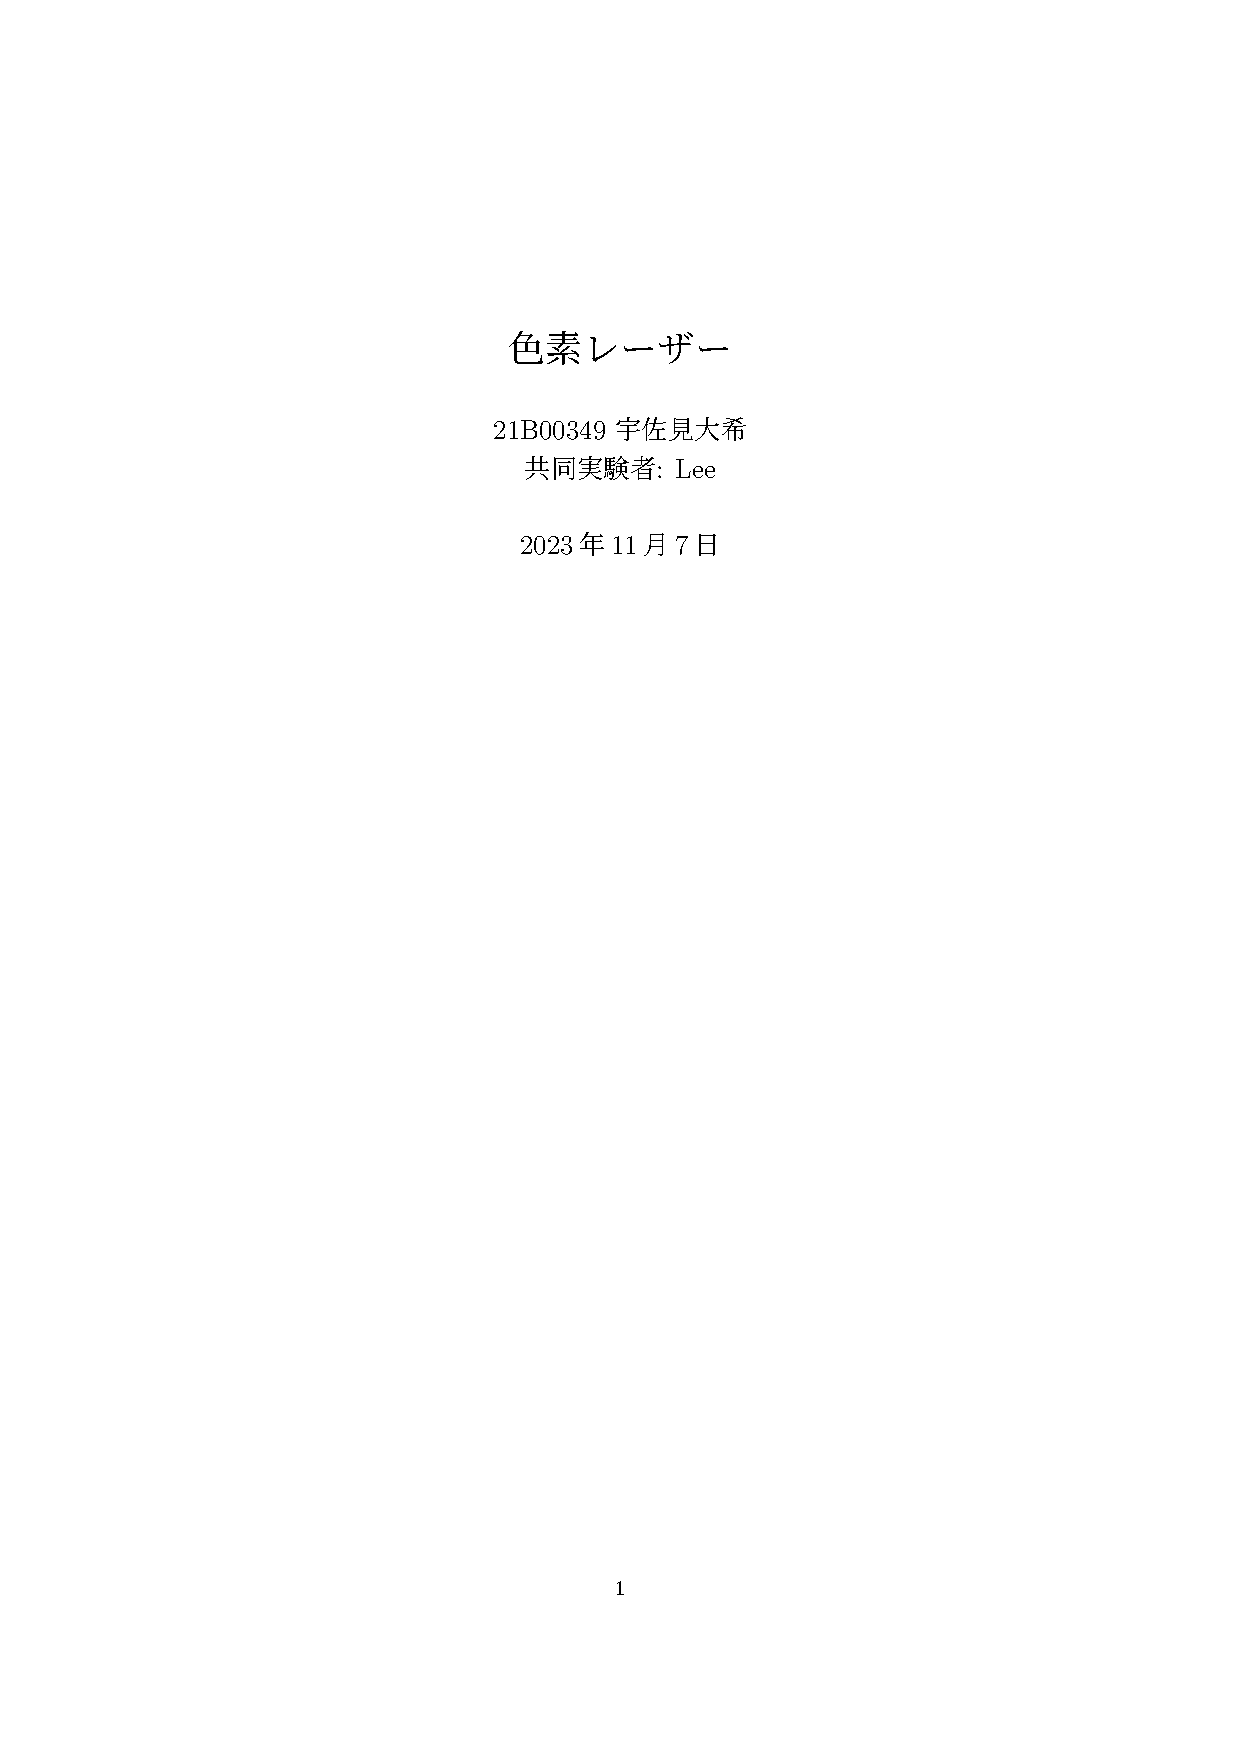
\includegraphics[width=8cm]{./assets/dye_laser.png}
    \caption{色素レーザーのスペクトル}
    \label{dye laser}
  \end{minipage}
\end{figure}

\begin{figure}[htbp]
  \centering
  \includegraphics[width=12cm]{./assets/flush_lamp_oscillo.jpg}
  \caption{フラッシュランプの時間波形}
  \label{flush lamp oscillo}
\end{figure}
\begin{figure}[htbp]
  \begin{minipage}[b]{0.5\linewidth}
    \centering
    \includegraphics[width=8cm]{./assets/fluorescence_oscillo.jpg}
    \caption{蛍光の時間波形}
    \label{fluorescene oscillo}
  \end{minipage}
  \begin{minipage}[b]{0.5\linewidth}
    \centering
    \includegraphics[width=8cm]{./assets/dye_laser_oscillo.jpg}
    \caption{色素レーザーの時間波形}
    \label{dye laser oscillo}
  \end{minipage}
\end{figure}

偏光特性についてはフラッシュランプ、蛍光、色素レーザー光のどれも見つけられなかった。
(課題 2.2.4) \\

\subsection{波長可変色素レーザーの実験}

最も出力が強くなる発振波長において発振するための放電電圧の閾値は 3.5 \si{V} となった。
これはプリズムによって波長を選択することによって課題 2.2.1 に比べて光量が減っているから必要な電圧が高まっていると考えられる。
(課題 3.1.1) \\

分光器を用いてプリズムの傾きを変えたときの色素レーザー光の波長のピークを調べる。
このとき最強となる波長は 600 \si{nm} で発振の成功率が 50 \% となる最短と最長の波長はそれぞれ 588 \si{nm}, 611 \si{nm} となった。
課題 2.2.2 の 600 \si{nm} の鋭いピークに対して 10\si{nm} ほど長短に拡がっている。
これは波長を選択することによって誘導放出がしやすくなったことによると考えられる。
(課題 3.1.2) \\

最も強い発振スペクトルは図 \ref{prism strongest} のようになった。プリズムを挟まなかった図 \ref{dye laser} と比べると線幅は変わらず、ピーク自体が振動しているように見える。 (課題 3.1.3) \\
\begin{figure}[htbp]
  \centering
  \includegraphics[width=12cm]{./assets/prism_strongest.png}
  \caption{最も強い発振スペクトル}
  \label{prism strongest}
\end{figure}

ここで共振器長 $l$ と共振器中で振動した周期数 $n$ を用いて波長 $\lambda_n$ とそれらの波長の間隔 $\Delta\lambda$ は次のように書ける。
\begin{align}
  \lambda_n     & = \frac{2l}{n}                                                                          \\
  \Delta\lambda & = \lambda_{n+1} - \lambda_n = 2l\ab(\frac{1}{n} - \frac{1}{n+1}) \approx \frac{2l}{n^2}
\end{align}
波長 $\lambda = 600\si{nm}$ 共振器長 $l = 3.0 \times 10^2\si{mm}$ であったので波長の間隔 $\Delta\lambda$ は次のようになる。
\begin{align}
  n             & = \frac{2l}{\lambda_n} = \frac{2\times 300\si{mm}}{600\si{nm}} = 1.0\times 10^6   \\
  \Delta\lambda & = 2\times 300\si{mm}\times\frac{1}{(1.0\times 10^6)^2} = 6.0\times 10^{-4}\si{nm}
\end{align}
これより $6.0\times 10^{-4}\si{nm}$ ごとに共振する。
\begin{align}
  m & = \frac{\lambda_{\max} - \lambda_{\min}}{\Delta\lambda} = \frac{23\si{nm}}{6.0\times 10^{-4}\si{nm}} = 3.83\times 10^4
\end{align}
更に $3.8\times 10^4$ 個程度のモード数がある。
(課題 3.1.4, 0.1.3) \\

最も強く発振する波長での時間波形は図 \ref{dye laser prism oscillo} のようになった。
これは図 \ref{dye laser oscillo} に比べて色素レーザー光の強度が弱くなっている。
(課題 3.1.5) \\
\begin{figure}[htbp]
  \centering
  \includegraphics[width=12cm]{./assets/dye_laser_prism.jpg}
  \caption{プリズムを通した色素レーザーの時間波形}
  \label{dye laser prism oscillo}
\end{figure}

偏光フィルターがある特定の角度で光強度がゼロとなるような偏光特性があった。
s 偏光はどんな角度でも光強度があり、偏光特性はあまり見られない。
それに対し p 偏光は約 60\textdegree で光強度がゼロとなるため、偏光板がその傾きのときそれから出てくる光強度はゼロとなる。
これより課題 2.2.4 は s 偏光、課題 3.1.6 は p 偏光と対応することがわかる。
(課題 3.1.6) \\

色素レーザー光は距離 1.7\si{m} に対して半径は $6\si{mm}$ となった。これより立体角 $\Omega$ は次のようになる。
\begin{align}
  \Omega = 4\pi\frac{\pi r^2}{\pi R^2} = 4\pi\frac{6^2}{1700^2} = 4\pi\times 1.2\times 10^{-5}
\end{align}
これより立体角 $4\pi$ の比は $1.2\times 10^{-5}$ となった。
(課題 3.1.7) \\

共振器長は $l = 300\si{mm}$ であるから往復数は次より 1.18 回であることがわかる。
\begin{align}
  \frac{1700 \si{mm}}{12 \si{mm}}\times 5\si{mm} & \approx 708.3\si{mm} \\
  \frac{708.3\si{mm}}{2l}                        & \approx 1.18
\end{align}
ミラーの反射率から考えるに反射可能な往復回数は 4.48 回であることがわかる。
\begin{align}
  \frac{1}{e} & = \ab(\frac{4}{5})^x \\
  x           & \approx 4.48
\end{align}
またフラッシュランプが光ってから発振するまでに $2.1\si{\mu s}$ 掛かったことから 1050 回往復していることがわかる。
\begin{align}
  \frac{c\Delta t}{2l} = \frac{3.0\times 10^8\si{m} \times 2.1\si{\mu s}}{2\times 300\si{mm}} = 1050
\end{align}
これらを総合してビームの拡散が一番大きく反射回数に影響する。
(課題 3.1.8) \\

色素レーザー光 1 パルスのエネルギー $V_{\mathrm{sum}}$ を三角形で近似すると
\begin{align}
  V_{\mathrm{sum}} & = 2.5\si{V} \times 4.0\si{\mu s} \times \frac{1}{2} = 5.0\times 10^{-6}\si{V\cdot s}
\end{align}
より光子数 $n_p$ については次のようになる。
\begin{align}
  V_{\mathrm{sum}} & = n_p \times\frac{\pi r^2}{2\pi l^2}\times \alpha eR                                                                    \\
                   & = n_p \times\frac{(2.5 \si{mm})^2}{2\times (40\si{mm})^2}\times 0.78\times 1.602\times 10^{-19}\si{C}\times 50\si{\ohm} \\
                   & = 1.95\times 10^{-19}\times n_p                                                                                         \\
  n_p              & = 2.56\times 10^{13}
\end{align}
よって色素レーザー光 1 パルス当たり $2.6\times 10^{13}$ 個の光子数が発射される。
(課題 3.1.9) \\

1 モード当たりの増幅率 $A$ は次のようになる。
\begin{align}
  A & = \ab(\frac{n_p}{m})^{\frac{1}{n}}                                 \\
    & = \ab(\frac{2.56\times 10^{13}}{3.84\times 10^4})^{\frac{1}{4.48}} \\
    & = 93.2
\end{align}
よって 1 パルスあたりの光の増幅率は 93 倍となる。
(課題 3.1.10) \\

\section{参考文献}
Neon
https://www.oceaninsight.jp/Products/2series.html


\end{document}